\chapter{Opis implementacji}
\label{Chapter6}

\section{Wstęp}
\label{Chapter61}

{\color{red}Wersja bez redakcji.}

%Wprowadzenie. Struktura tego rozdziału nie jest z góry określona, gdyż mocno zależy to od specyfiki projektu. Generalnie w poszczególnych podrozdziałach każdy powinien opisać swoją część z takiego technicznego punktu widzenia. Piszecie, jak zrealizowaliście poszczególne wymagania, jak to wygląda ,,pod maską'', oczywiście też trzeba przyjąć jakiś poziom szczegółowości. W bardzo szczególnych przypadkach chyba może się zdarzyć, że trzeba będzie załączyć fragment jakiegoś kodu źródłowego czy konfiguracji -- generalnie ma to być opisane w taki sposób, że jako osoba nieznająca systemu siadam i wiem, jak i co zrobiliście. Oczywiście, to moje dywagacje, być może osoby związane z uczelnią zlinczują mnie za ten fragment.
%
\section{Użyte technologie}
\label{Chapter62}

\subsection{Moodle}
\emph{Moodle} (roz. \textit{Modular Object-Oriented Dynamic Learning Environment}) -- stanowi podstawę systemu \textit{iQuest}. Wyboru dokonano ze względu na kilka czynników:
\begin{itemize}
\item{Propozycję Architekta, wynikającą z faktu, iż Moodle posiada już implementację wielu wymaganych w \textit{iQuest} mechanizmów.}
\item{Oczekiwania Klienta, wynikające z popularności platformy Moodle wśród systemów uczelnianych.}
\end{itemize}

\subsection{PHP}
\emph{PHP} -- platforma Moodle opiera się właśnie na tym języku programowania. Z tego względu, jest to też technologia zastosowana w większości rozszerzeń utworzonych przez zespół /textit{iQuest}, korzystających z wielu interfejsów programowania aplikacji tej platformy.

\subsection{PHPUnit}
Ze względu na fakt, iż programiści \textit{Moodle'a} wykonują testy jednostkowe kodu wykorzystując do tego celu \emph{PHPUnit}, zdecydowano o wzorowaniu się na tym działaniu. \textit{Moodle} udostępnia dwie klasy do testowania -- \textit{basic\_testcase} i \textit{advanced\_testcase}, przy czym ta druga służy do testów, które wchodzą w interakcję z bazą danych.

\subsection{Selenium}
\emph{Selenium} -- szybko rozwijające się narzędzie do testów akceptacyjnych. Był to naturalny wybór zwłaszcza, że zostało ono przybliżone zespołowi \textit{iQuest} na zajęciach z Inżynierii Oprogramowania w trakcie toku studiów.

\subsection{PostgreSQL}
System zarządzania bazą danych \emph{PostgreSQL} został wybrany ze względu na wymagania pozafunkcjonalne.

\subsection{Eclipse IDE}
Wybór \emph{Eclipse IDE} jako stosowanego dla projektu \textit{iQuest} zintegrowanego środowiska programistycznego wynika z faktu, iż oprogramowanie to jest dostępne za darmo. Dodatkową zaletą \textit{Eclipse} jest modularność tego rozwiązania, dzięki czemu dostępny jest w nim dodatek \emph{PHP Development Tools}, znacząco upraszczający pracę z technologią PHP.

\subsection{SVN}
\emph{Subversion} został wybrany jako podstawowy system zarządzania treścią ze względu na wymagania pozafunkcjonalne. Dodatkową zaletą jego użycia jest fakt, że zespół eksploatacji, który docelowo przejmie zarządzanie artefaktami związanymi z projektem, wykorzystuje właśnie \textit{SVN}.

\subsection{Redmine}
Systemu zarządzania projektami \emph{Redmine} wykorzystywany był od samego początku istnienia projektu. Jest to narzędzie bardzo przydatne w wymianie informacji pomiędzy członkami zespołu, integrujące się m.in. z repozytorium kodu. Technologia ta została narzucona, ze względu na sposób organizacji pracy w \textit{Software Development Studio} na Politechnice Poznańskiej.

\subsection{JasperReports}
Ze względu na wymagania pozafunkcjonalne, zdecydowano się skorzystać z mechanizmów raportowania oferowanych przez \emph{JasperReports}.

%MT
\subsection{JavaScript}
Formularze wymagające częstej interakcji z klientem, np. formularz umożliwiający tworzenie nowej ankiety, oraz funkcje związane z walidacją pól uzupełnianych przez klienta zostały napisane w \emph{JavaScript}. Obsługa strony po stronie użytkownika zapobiega frustracji, związanej z częstym przeładowywaniem całej strony, co ogranicza zarówno obciążenie łącza po stronie serwera, jak i po stronie klienta.

\section{Ogólna struktura projektu}
\label{Chapter63}

{\color{red}Sekcja druga.}

\section{Interfejs}
\label{Chapter64}

\subsection{Wprowadzenie}
Jedną z części pracy było zaprojektowanie graficznego interfejsu użytkownika. Głównym problemem jaki się pojawił, był wybór odpowiedniego narzędzia. Celem jaki postawiono, była maksymalna zgodność projektowanych elementów z różnymi wersjami \emph{Moodle} -- zarówno wcześniejszymi, jak i późniejszymi. Zdecydowano, aby starać się korzystać z gotowych interfejsów programowania aplikacji \emph{(API)} dostarczonych przez \emph{Moodle}, tj. \emph{Page API}, \emph{Form API}, oraz \emph{Access API}. Wszystkie interfejsy są napisane przy użyciu języka PHP -- są wykonywane po stronie serwera. Konieczne okazało się też wykonanie niektórych skryptów po stronie klienta. Dlatego w projekcie wykorzystano również język skryptowy \emph{Java Script}.

\section{Logika (back-end)}
\label{Chapter65}

Jednym z zadań w ramach pracy było zaprogramowanie odpowiedniej logiki biznesowej rozwiązującej zadania stawiane przed zaprojektowanym systemem. Najważniejszym zadaniem z perspektywy back-end'u jest interakcja z bazą danych. Poza tym system posiada: procesor zadań wykonywanych w tle oparty na \emph{cron}; moduł odpowiadający za komunikację z systemem uczelanianym \emph{ePoczta}; moduł logowania zdarzeń. W trakcie implementacji zdecydowano się nie tworzyć osobnego mechanizmu do przechowywania ustawień w bazie danych i skorzystaliśmy z istniejącego już w \emph{Moodle}. Jednym z wymagań pozafunkcjonalnych było wykorzystanie bazy danych \emph{PostgreSQL}. Platforma \emph{Moodle} korzysta z mechanizmu \emph{XMLDB}, co pozwala na ominięcie wielu problemów pojawiających się przy migracjach pomiędzy różnymi systemami baz danych. Niestety kosztem wykorzystania tego mechanizmu jest konieczność pracy z interfejsami programowania aplikacji dostarczanymi przez platformę \emph{Moodle}, m.in. \emph{Data manipulation API} (zarządzanie danymi), \emph{Access API} (zarządzanie dostępem, rolami, prawami).\\

{\color{red} Część do rozszczepienia w inne obszary}
Poniżej przedstawiony został schemat bazy danych i logikę biznesową z perspektywy implementacyjnej.

\newpage
\begin{landscape}

\begin{figure}[!th]
\centering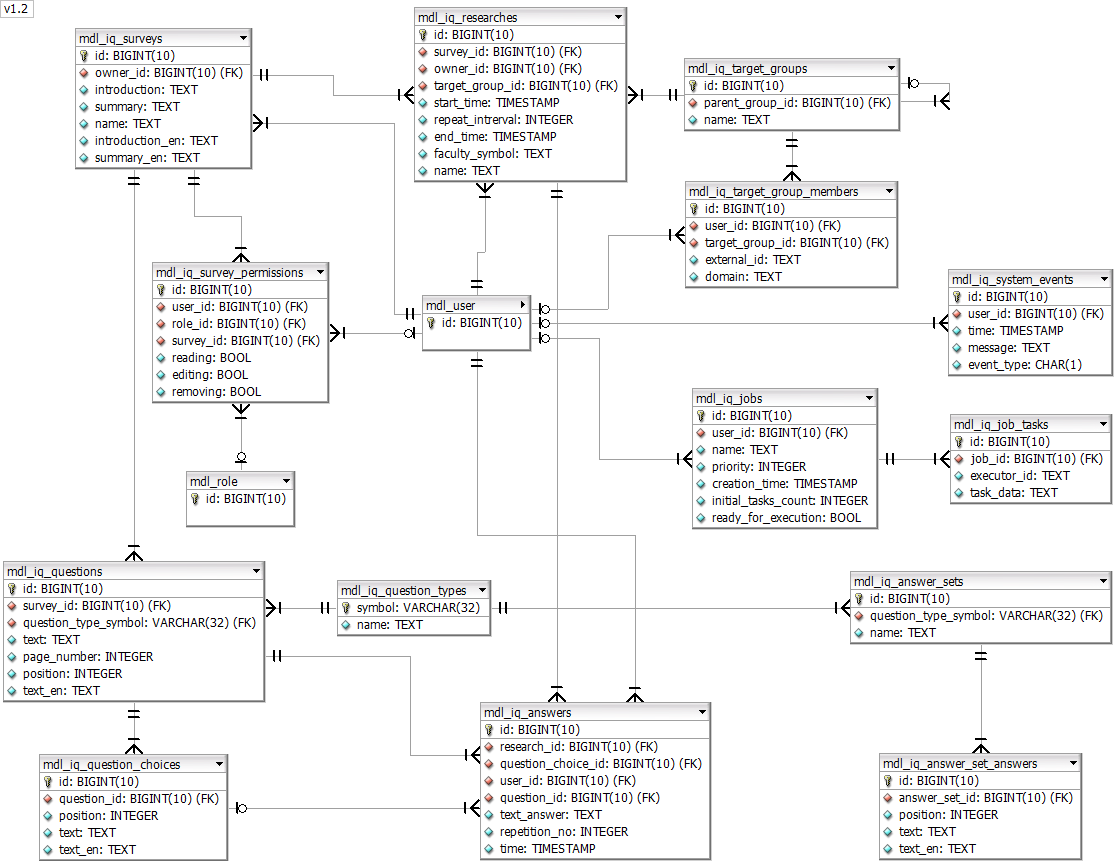
\includegraphics[width=1.25\textheight]{figures/iQuest_Database.png}
\caption{Backend -- Schemat bazy danych}\label{rys:iquest-db}
\end{figure}

\begin{figure}[!th]
\centering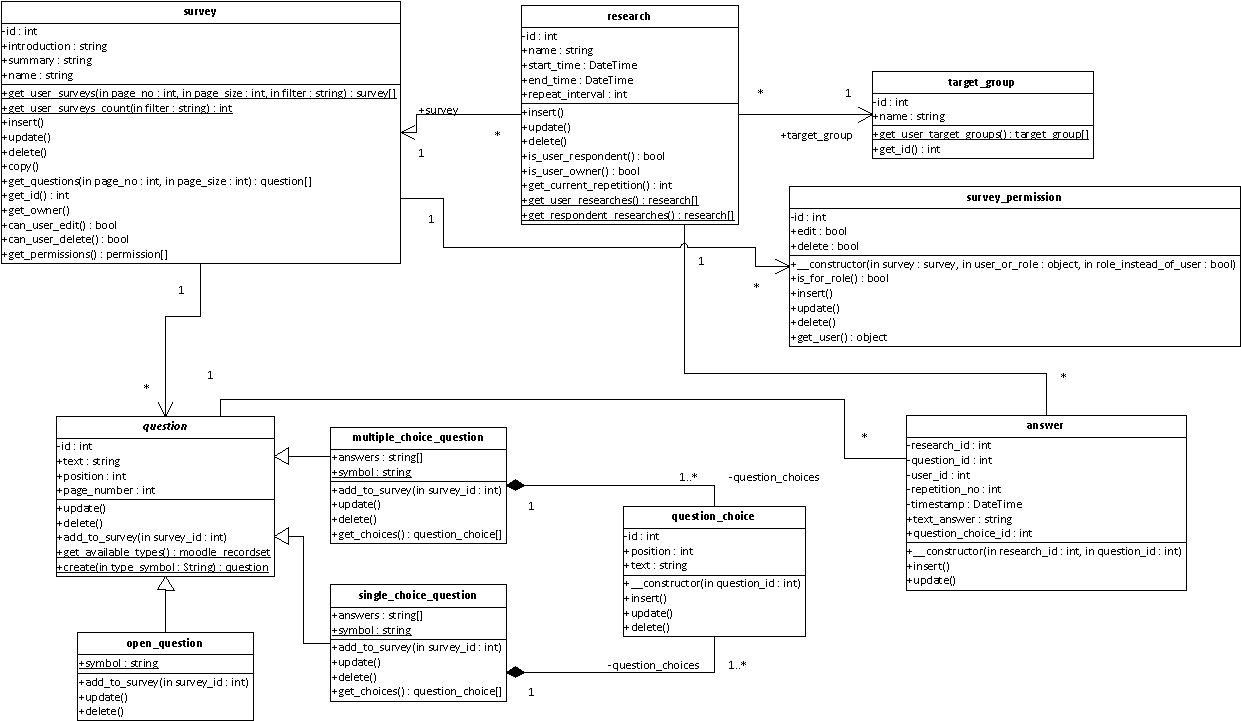
\includegraphics[width=1.25\textheight]{figures/Survey_Creator_Survey_Runner.png}
\caption{Backend -- moduły Survey Creator i Survey Runner}\label{rys:iquest-backend}
\end{figure}

\begin{figure}[!th]
\centering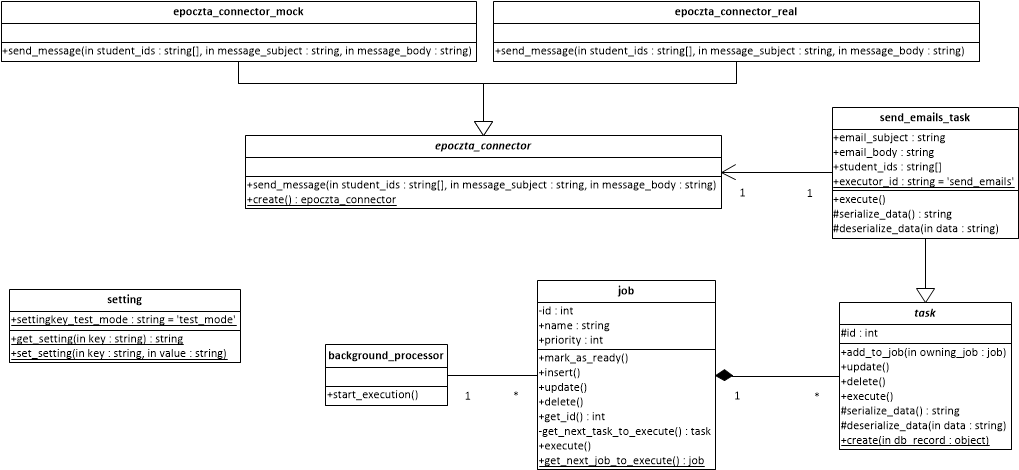
\includegraphics[width=1.25\textheight]{figures/ePoczta_Connector_Background_Task_Scheduler_and_Executor.png}
\caption{Backend -- moduły ePoczta Connector i Background Task Scheduler and Executor}\label{rys:iquest-backend2}
\end{figure}

\end{landscape}

\section{Powiązanie back-endu z interfejsem}
\label{Chapter66}

{\color{red}Dalsze opisy.}